\documentclass[journal,compsoc]{IEEEtran}
\usepackage{tikz}
\usetikzlibrary{arrows.meta,positioning,shapes.geometric,fit,calc,backgrounds}
\usepackage{xcolor}

\definecolor{tierclient}{RGB}{236,244,252}
\definecolor{tierclientborder}{RGB}{41,128,185}
\definecolor{tiergate}{RGB}{254,249,238}
\definecolor{tiergateborder}{RGB}{214,137,16}
\definecolor{tierfast}{RGB}{247,243,252}
\definecolor{tierfastborder}{RGB}{142,68,173}
\definecolor{tierdb}{RGB}{237,247,242}
\definecolor{tierdbborder}{RGB}{39,174,96}

\tikzset{
  cnode/.style={draw=#1, fill=white, rounded corners=3pt, line width=0.7pt, align=center},
  dnode/.style={draw=#1, cylinder, shape border rotate=90, aspect=0.25, fill=white, line width=0.7pt, align=center},
  arrow/.style={-{Stealth[length=2.2mm,width=1.5mm]}, line width=0.8pt, draw=black!75},
  darrow/.style={{Stealth[length=2mm,width=1.3mm]}-{Stealth[length=2mm,width=1.3mm]}, line width=0.8pt, draw=black!75},
  labeltext/.style={font=\tiny\bfseries, text=black!80}
}

\begin{document}

\begin{figure*}
\centering
\resizebox{0.96\textwidth}{!}{%
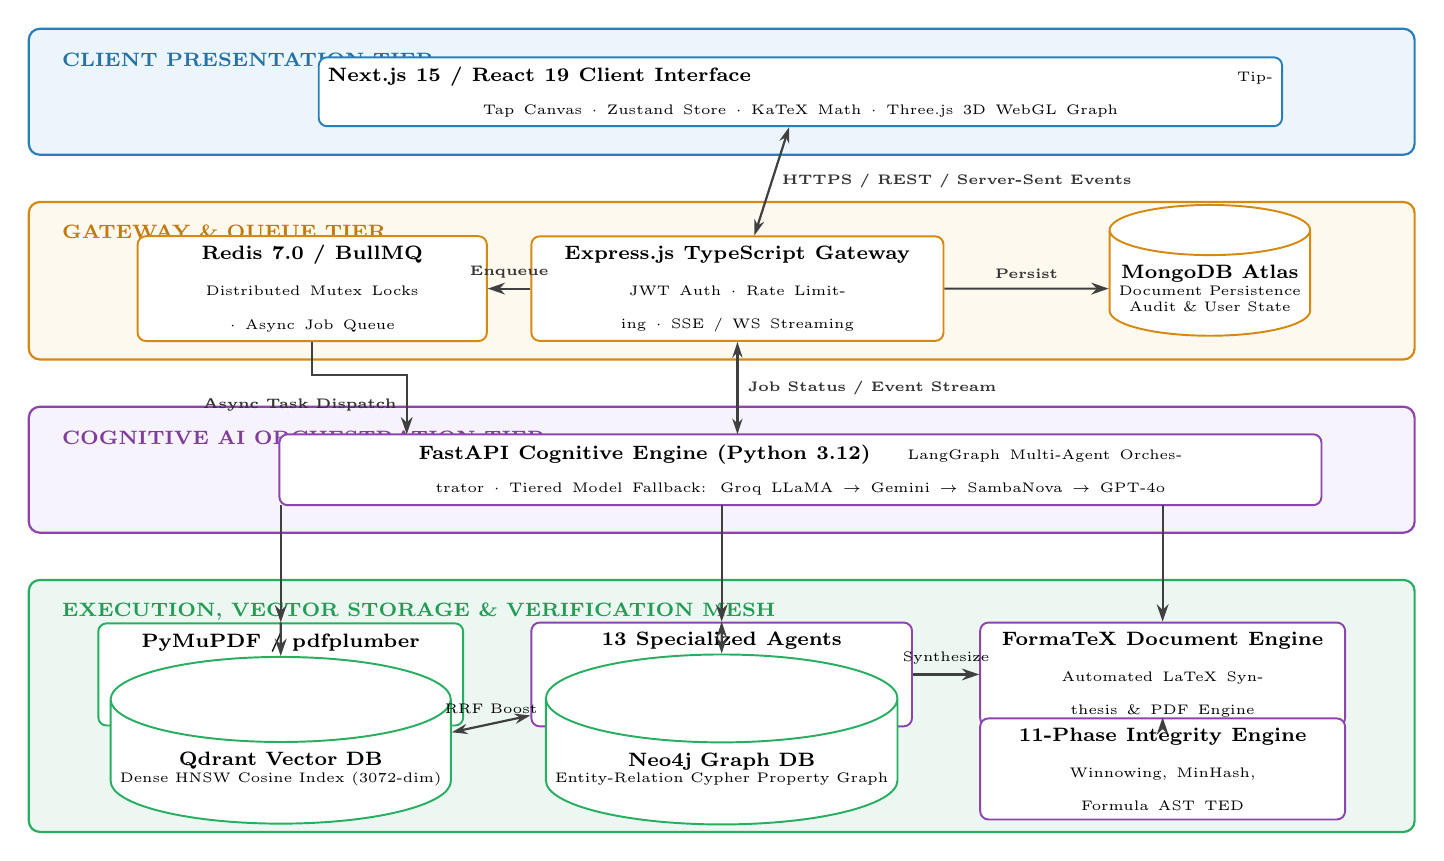
\begin{tikzpicture}[x=1mm, y=1mm]

% ==================== TIER 1: CLIENT TIER ====================
\draw[rounded corners=4pt, fill=tierclient, draw=tierclientborder, line width=0.8pt] (-88, 54) rectangle (88, 70);
\node[anchor=west, font=\scriptsize\bfseries, text=tierclientborder!90!black] at (-85, 66) {CLIENT PRESENTATION TIER};
\node[cnode=tierclientborder, text width=120mm, minimum height=8mm] (client) at (10, 62) {
  \textbf{\scriptsize Next.js 15 / React 19 Client Interface} \hfill \tiny TipTap Canvas $\cdot$ Zustand Store $\cdot$ KaTeX Math $\cdot$ Three.js 3D WebGL Graph
};

% ==================== TIER 2: GATEWAY & PERSISTENCE TIER ====================
\draw[rounded corners=4pt, fill=tiergate, draw=tiergateborder, line width=0.8pt] (-88, 28) rectangle (88, 48);
\node[anchor=west, font=\scriptsize\bfseries, text=tiergateborder!90!black] at (-85, 44) {GATEWAY \& QUEUE TIER};

\node[cnode=tiergateborder, text width=42mm, minimum height=11mm] (redis) at (-52, 37) {
  \textbf{\scriptsize Redis 7.0 / BullMQ}\\[1pt]
  \tiny Distributed Mutex Locks $\cdot$ Async Job Queue
};

\node[cnode=tiergateborder, text width=50mm, minimum height=11mm] (gateway) at (2, 37) {
  \textbf{\scriptsize Express.js TypeScript Gateway}\\[1pt]
  \tiny JWT Auth $\cdot$ Rate Limiting $\cdot$ SSE / WS Streaming
};

\node[dnode=tiergateborder, minimum width=24mm, minimum height=11mm, font=\tiny] (mongo) at (62, 37) {
  \textbf{\scriptsize MongoDB Atlas}\\
  Document Persistence\\
  Audit \& User State
};

% ==================== TIER 3: COGNITIVE AI ENGINE TIER ====================
\draw[rounded corners=4pt, fill=tierfast, draw=tierfastborder, line width=0.8pt] (-88, 6) rectangle (88, 22);
\node[anchor=west, font=\scriptsize\bfseries, text=tierfastborder!90!black] at (-85, 18) {COGNITIVE AI ORCHESTRATION TIER};

\node[cnode=tierfastborder, text width=130mm, minimum height=9mm] (fastapi) at (10, 14) {
  \textbf{\scriptsize FastAPI Cognitive Engine (Python 3.12)} \quad
  \tiny LangGraph Multi-Agent Orchestrator $\cdot$ Tiered Model Fallback: Groq LLaMA $\to$ Gemini $\to$ SambaNova $\to$ GPT-4o
};

% ==================== TIER 4: REASONING, STORAGE & VERIFICATION MESH ====================
\draw[rounded corners=4pt, fill=tierdb, draw=tierdbborder, line width=0.8pt] (-88, -32) rectangle (88, 0);
\node[anchor=west, font=\scriptsize\bfseries, text=tierdbborder!90!black] at (-85, -4) {EXECUTION, VECTOR STORAGE \& VERIFICATION MESH};

% Column 1: Ingest & Vector
\node[cnode=tierdbborder, text width=44mm, minimum height=10mm] (ingest) at (-56, -12) {
  \textbf{\scriptsize PyMuPDF / pdfplumber}\\[1pt]
  \tiny Layout-Aware Ingestion \& Math Extraction
};
\node[dnode=tierdbborder, minimum width=26mm, minimum height=10mm, font=\tiny] (qdrant) at (-56, -24) {
  \textbf{\scriptsize Qdrant Vector DB}\\
  Dense HNSW Cosine Index (3072-dim)
};

% Column 2: Multi-Agent & Knowledge Graph
\node[cnode=tierfastborder, text width=46mm, minimum height=10mm] (agents) at (0, -12) {
  \textbf{\scriptsize 13 Specialized Agents}\\[1pt]
  \tiny Planner, Researcher, Fact-Check, Reviewer...
};
\node[dnode=tierdbborder, minimum width=26mm, minimum height=10mm, font=\tiny] (neo4j) at (0, -24) {
  \textbf{\scriptsize Neo4j Graph DB}\\
  Entity-Relation Cypher Property Graph
};

% Column 3: FormaTeX & Academic Integrity
\node[cnode=tierfastborder, text width=44mm, minimum height=10mm] (formatex) at (56, -12) {
  \textbf{\scriptsize FormaTeX Document Engine}\\[1pt]
  \tiny Automated LaTeX Synthesis \& PDF Engine
};
\node[cnode=tierfastborder, text width=44mm, minimum height=10mm] (integrity) at (56, -24) {
  \textbf{\scriptsize 11-Phase Integrity Engine}\\[1pt]
  \tiny Winnowing, MinHash, Formula AST TED
};

% ==================== ARROWS ====================
% Tier 1 <-> Tier 2
\draw[darrow] (client) -- node[right, labeltext] {HTTPS / REST / Server-Sent Events} (gateway);

% Tier 2 internal
\draw[arrow] (gateway) -- node[above, labeltext] {Enqueue} (redis);
\draw[arrow] (gateway) -- node[above, labeltext] {Persist} (mongo);

% Tier 2 -> Tier 3
\draw[arrow] (redis) -- ++(0,-11) -| node[near end, left, labeltext] {Async Task Dispatch} (-40, 18.5);
\draw[darrow] (gateway) -- node[right, labeltext] {Job Status / Event Stream} (2, 18.5);

% Tier 3 -> Tier 4
\draw[arrow] (-56, 9.5) -- (ingest);
\draw[arrow] (0, 9.5) -- (agents);
\draw[arrow] (56, 9.5) -- (formatex);

% Tier 4 vertical connections
\draw[arrow] (ingest) -- (qdrant);
\draw[darrow] (agents) -- (neo4j);
\draw[darrow] (agents) -- node[above, font=\tiny] {RRF Boost} (qdrant);
\draw[arrow] (agents) -- node[above, font=\tiny] {Synthesize} (formatex);
\draw[arrow] (formatex) -- (integrity);

\end{tikzpicture}}
\caption{Distributed architecture of ResearcherGPT across client, gateway, cognitive orchestration, and storage mesh tiers.}
\end{figure*}

\end{document}
